\chapter{Utility Designer}
\label{chap:utilitydesigner}
\section{Introduction}
\label{sec:utilitydesigner_introduction}

There are many solutions available for creating AIs, and it is important for developers to have a good set of tools. At the moment there are some really good assets in the Unity Asset Store for FSMs and behaviour trees, as the concept has been around for a long time. However, for implementations of more dynamic behaviours, such as utility AI, there is not as much to be found.

The tool developed in this thesis, called Utility Designer, aims to fill this gap by providing a generic and intuitive tool that uses a combination of utility AI and behaviour trees. Utility AI is used to decide the best state, where each state has a behaviour tree that defines the specific actions and behaviours of that state. This combination allows the NPC to make decisions on their own, while still being able to define the execution of states with familiar behaviour trees.

A crucial aspect of designing a tool for others is to effectively communicate how it works, as users may have no prior knowledge of it. Not only is it important to keep the tool simple by hiding complex structures behind an intuitive and pleasing interface, but it must also provide a quick way for a new user to learn how it works. This is a key component of any tool, as its purpose is to save programmers time by doing some of the work for them. It is therefore essential to provide a manual, sample scenes, a tutorial video, etc.

A manual explaining everything about Utility Designer can be found in the appendix to learn more about how the tool works.

\section{Use Cases}
\label{sec:utilitydesigner_usecases}

The ideal use case is where NPCs need to make dynamic decisions based on the current situation, where they cannot simply follow fixed rules. It thrives when multiple factors influence an NPC's behaviour and decision-making process. Here are some different use cases for Utility Designer:

\paragraph{Expandability:}
When making a game or simulation, sometimes new features are added that give NPCs a new state to choose from, such as the option to go swimming. In Utility Designer, adding a new state is enough for the NPC to include it in their decision making. There is no dependency on the complexity of the structure and the amount of choices the NPC has, because all the other states do not need to be touched when you add a new one. Doing something like this in a state machine or behaviour tree might not be so straightforward.

\paragraph{Built-in Behaviour Tree:}
In a situation where utility AI is not required, for example when creating sequential behaviour for a tour guide, Utility Designer offers the option of using the tool as a normal behaviour tree. This can be achieved by simply using one state without any preconditions and then using its behaviour tree to create the desired behaviour. This behaviour tree will then always be executed as it is the only state that can be selected.

\paragraph{Multiple NPCs:}
If there is a need to create multiple instances of the same character, NPCs with a Utility Designer component on them can simply be copied and pasted, or instantiated from a prefab. They will then share the same behaviour rules, which can be useful for something like a group of monsters.

\paragraph{Dynamic Environments:}
In video games or simulations where things change a lot, utility AI helps NPCs make good decisions. They check things like how close enemies are, if there are resources nearby, or what's happening at important locations. The decisions are then made by the NPCs themselves, which makes them feel more real.

\paragraph{Easy To Adjust:}
Imagine a scenario where a small village should be populated with different kinds of NPCs to make the village feel alive to the player. Most states are shared by all the NPCs, such as "Sleep", "Eat", "Read newspaper" "Walk around", "Talk" and so on. These states only need to be created once and can then be used by any NPC. The behaviour can then be copied, and a few weights or states can be changed, making it incredibly easy to create unique personalities for different characters. One of them might for example be an introvert, and have their weights for "Walk around" and "Talk" a bit lower, while the state "Read newspaper" is weighted more.

\section{Implementation}
\label{sec:utilitydesigner_implementation}

\subsection{Technology Stack}
\label{sec:utilitydesigner_implementation_technologystack}

\subsubsection{Overview}
\label{sec:utilitydesigner_implementation_technologystack_overview}

The Utility Designer uses different technologies to facilitate a synergistic relationship between utility AI and behaviour trees, simplifying the process of generating advanced and dynamic behaviours. Unity and C\# have both been around for some time, making them mature and well-established technologies. Despite their longevity, they are still actively maintained and updated to reflect new advances in software development. Unity's UI toolkit, on the other hand, is relatively new and continues to be actively developed.

\subsubsection{Unity}
\label{sec:utilitydesigner_implementation_technologystack_unity}

Unity is the base layer of the tool. Utility Designer is built in Unity because Unity's Asset Store is a good way to share tools and assets with other developers. The latest version of Unity used is 2022, as each version adds more features to the UI toolkit, and it's the latest stable release to date. This cross-platform game engine is used as the basis for all development activities. Robust, feature-rich and versatile, Unity serves as the cornerstone in the creation and operation of the Utility Designer, handling everything from 3D environment rendering and user input management to game physics.

\subsubsection{C\#}
\label{sec:utilitydesigner_implementation_technologystack_csharp}

The core logic of Utility Designer is written in C\#, a powerful object-oriented programming language. C\# is used to implement the utility's AI and behaviour tree logic, and to manage interactions with the user interface. This programming language provides access to a wide range of libraries and features, allowing a high degree of customisation and control over the project structure.

\subsubsection{Unity's UI Toolkit}
\label{sec:utilitydesigner_implementation_technologystack_unitysuitoolkit}

Unity provides a system for creating editor windows called UI Toolkit. It is used to create a visually appealing and interactive user interface. The UI Toolkit is a flexible and efficient system for building UI in Unity and is used to create a rich, yet simple and user-friendly graphical interface for the Utility Designer. The toolkit allows the UI to be designed using UXML and USS, languages similar to HTML and CSS respectively, allowing for highly flexible and scalable UI design.

\subsection{Software Architecture}
\label{sec:utilitydesigner_implementation_softwarearchitecture}

The architecture of Utility Designer has been designed so that it has no dependencies outside of its own folder, allowing the folder to be freely moved around without any problems. In addition, users do not need to interact with or write scripts within this folder, and its own assembly definition ensures that the tool remains self-contained.

Splitting the code into different namespaces significantly reduces dependencies throughout the project, making it easier to maintain. Three particular namespaces stand out as the most important.

\begin{tabular}{lp{12cm}}
Evaluation: & This namespace contains the functionality for the evaluation tab and implements the logic and calculations of utility AI, as well as the considerations. \cr
Execution: & Used for the implementation of the behaviour tree found in the execution tab. It also contains all the various predefined nodes and the SceneReferences script. \cr
Editor: & Here are all the UXML and USS documents needed to visualise the different editor windows, as well as some C\# scripts to add logic such as user interaction and runtime debugging. This folder is ignored by Unity during runtime builds to save resources.
\end{tabular}

Outside of these namespaces is the UtilityDesigner script which holds the logic to initialise and update the evaluation and execution tab according to the specified tick rate. It is also responsible for the safe, load and log functions.

The design of the tool is not focused on optimising the example scenes. Furthermore, these scenes are not housed within the UtilityDesigner assembly, but are external to it, as they are not directly related to the core functionality of the tool. They simply use Utility Designer from an external position, reflecting the scenario of a developer who has included Utility Designer in their project as a standalone tool to increase production speed.

\subsection{Discarded Concepts}
\label{sec:utilitydesigner_implementation_discardedconcepts}

Developing tools can sometimes be tricky, especially when doing it for the first time, because a tool like Utility Designer has to provide different aspects for the developer to speed up their production, while still remaining generic, intuitive and maintainable. Therefore, some concepts were not completely clear from the start. Different approaches were tested to find the best one.

\paragraph{Scene References:}
One of the key decisions was to store the behaviour as a ScriptableObject, making it easy to maintain as it can be duplicated and freely attached and removed from the UtilityDesigner script. One of the characteristics of ScriptableObjects is that no references from the scene can be stored in them. However, it is important for the action nodes to have access to references from the scene, such as the location of the NPC's house or the enemy. Hence the concept of the SceneReferences script. But before that, there were other ideas to solve this problem:

\begin{tabular}{lp{12cm}}
Inspector: & The most intuitive way would be to drag and drop the references to the node inspector. As these references cannot be saved in the ScriptableObject, the name of the GameObject could be stored instead as a workaround. However, this creates a problem if two or more of these references have the same name, as they can no longer be clearly distinguished by name alone. And trusting the user not to give the same name to two GameObjects in their scene that are used in a behaviour tree is too risky. \cr
Event manager: & Instead of making action nodes based on separate scripts, another approach could be to have a static event manager. The user could then subscribe to events from the manager, and these events would be fired each time the action node is invoked. The problem with this approach is that the main advantage of action scripts is lost: the ability to re-use the same code for different behaviours with the click of a button. It also makes it difficult to encapsulate parts of the code with a single giant event manager, which could make the code organisation of a large project worse.
\end{tabular}

Considering these ideas, the best approach was to create a script called SceneReferences, which contains all the references needed for a UtilityDesigner. This script can then be attached to a GameObject in the scene and the name of the GameObject is stored in the ScriptableObject. References from SceneReferences can then be easily accessed in the action nodes in the node inspector or through a provided API. This makes it possible to have separate scripts for the action nodes without having to trust the end user. SceneReferences are not restricted to the behaviour tree and can be used elsewhere in the project.

\newpage

\paragraph{Execution Tab:}
It was not clear from the start what the execution tab would look like, and different ideas were considered depending on the time available for implementation:

\begin{tabular}{lp{10cm}}
Link other implementations: & If there was no time for the execution tab, there should at least have been a way to link to other assets, such as a behaviour tree asset. Fortunately, there was enough time to implement a useful framework. \cr
State Machine: & The first idea used was an implementation of a state machine, because it is quite easy to implement. But the more the tool was tested, the more it became clear that loops are used very often in the execution tab, and state machines are not the best thing for that, as shown in the section \ref{sec:projectevolution_whyitfails}. \cr
Behaviour Tree: & Since there was still time for a more complex framework, and the scene reference problem wasn't solved yet, it seemed like a good opportunity to start implementing a behaviour tree. They are very flexible and well known among AI developers, which makes it easier for them to get started with Utility Designer. \cr
GOAP: & Goal Oriented Action Planning could also be a possible approach for executing states, as the evaluation tab could decide the goal, and GOAP would plan how to execute it. The problem is that GOAP is harder to get started with than BTs, and in many cases a simple sequence of actions is sufficient for a state, making the added complexity of GOAP unnecessary.
\end{tabular}

\begin{figure}[H]
	\centering
		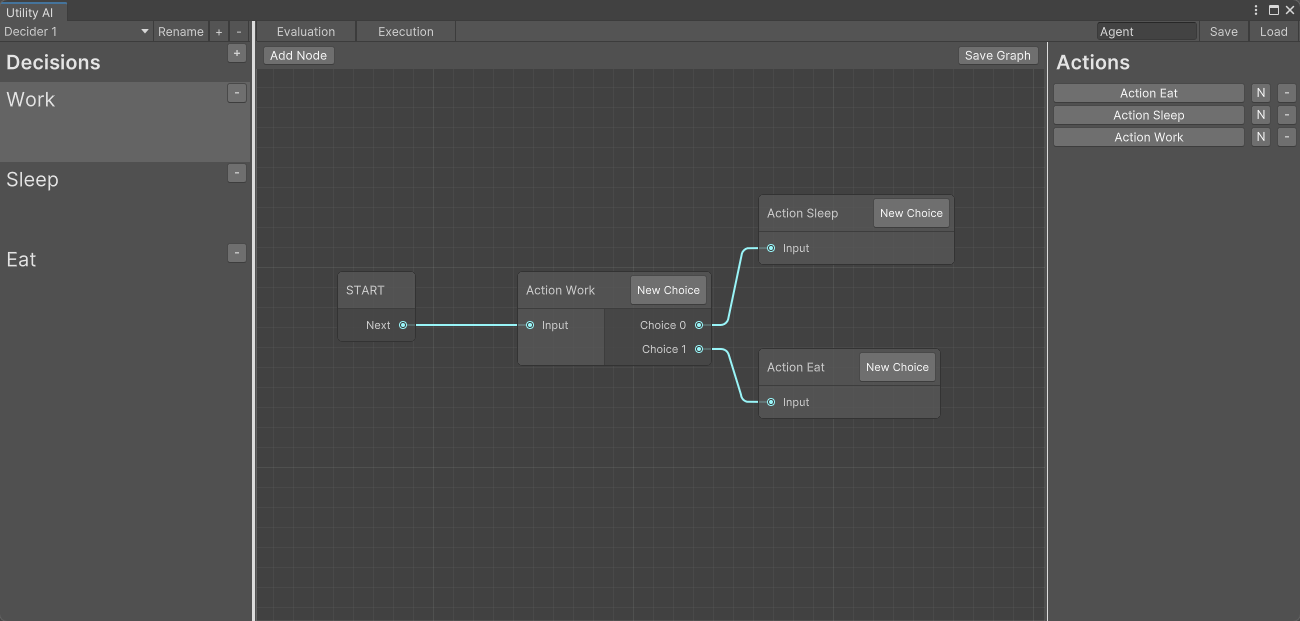
\includegraphics[scale=0.38]{images/utility_designer_state_machine.png}
	\caption{Discarded implementation of a state machine}
	\label{fig:utility_designer_state_machine}
\end{figure}

However, there is always the option to use a custom framework to execute nodes, simply by using an action node in the execution tab, which then calls the external framework to execute the state.

\newpage

\subsection{Third Party Code}
\label{sec:utilitydesigner_implementation_thirdpartycode}

In order to speed up the development process and achieve more goals, the help of some external tools and websites have been included. Extensive research was conducted across multiple websites such as Unity's documentation (Unity Docs)\footnote{\url{https://docs.unity.com}}, YouTube tutorials, especially this one for the behaviour tree (YouTube)\footnote{\url{https://youtu.be/nKpM98I7PeM}} and (Stack Overflow)\footnote{\url{https://stackoverflow.com}}, among others.

In addition, the AI-powered tool, ChatGPT (ChatGPT)\footnote{\url{https://chat.openai.com}}, and the autocorrect functionality provided by JetBrains' IDE for C\#, known as Rider (JetBrains Rider)\footnote{\url{https://www.jetbrains.com/rider/}}, were instrumental in improving efficiency and code quality.

Apart from the author and supervisor of this thesis, no one else contributed to the code. However, it is worth noting that the basic idea of how utility AI is implemented comes from Project 2, the previous project before the thesis.

\section{Example Scenes}
\label{sec:utilitydesigner_implementation_examplescenes}
\subsection{Daily Routine}
\label{sec:utilitydesigner_implementation_examplescenes_dailyroutine}

The first and simpler example again shows an agent trying to live a normal daily routine. Everything is the same as in section \ref{subsec:utilityai_realization_dailyroutine}, except that the house is white instead of blue, and the consideration saturation has been renamed to hunger to keep consistency with the second example scene.

\begin{figure}[H]
	\centering
		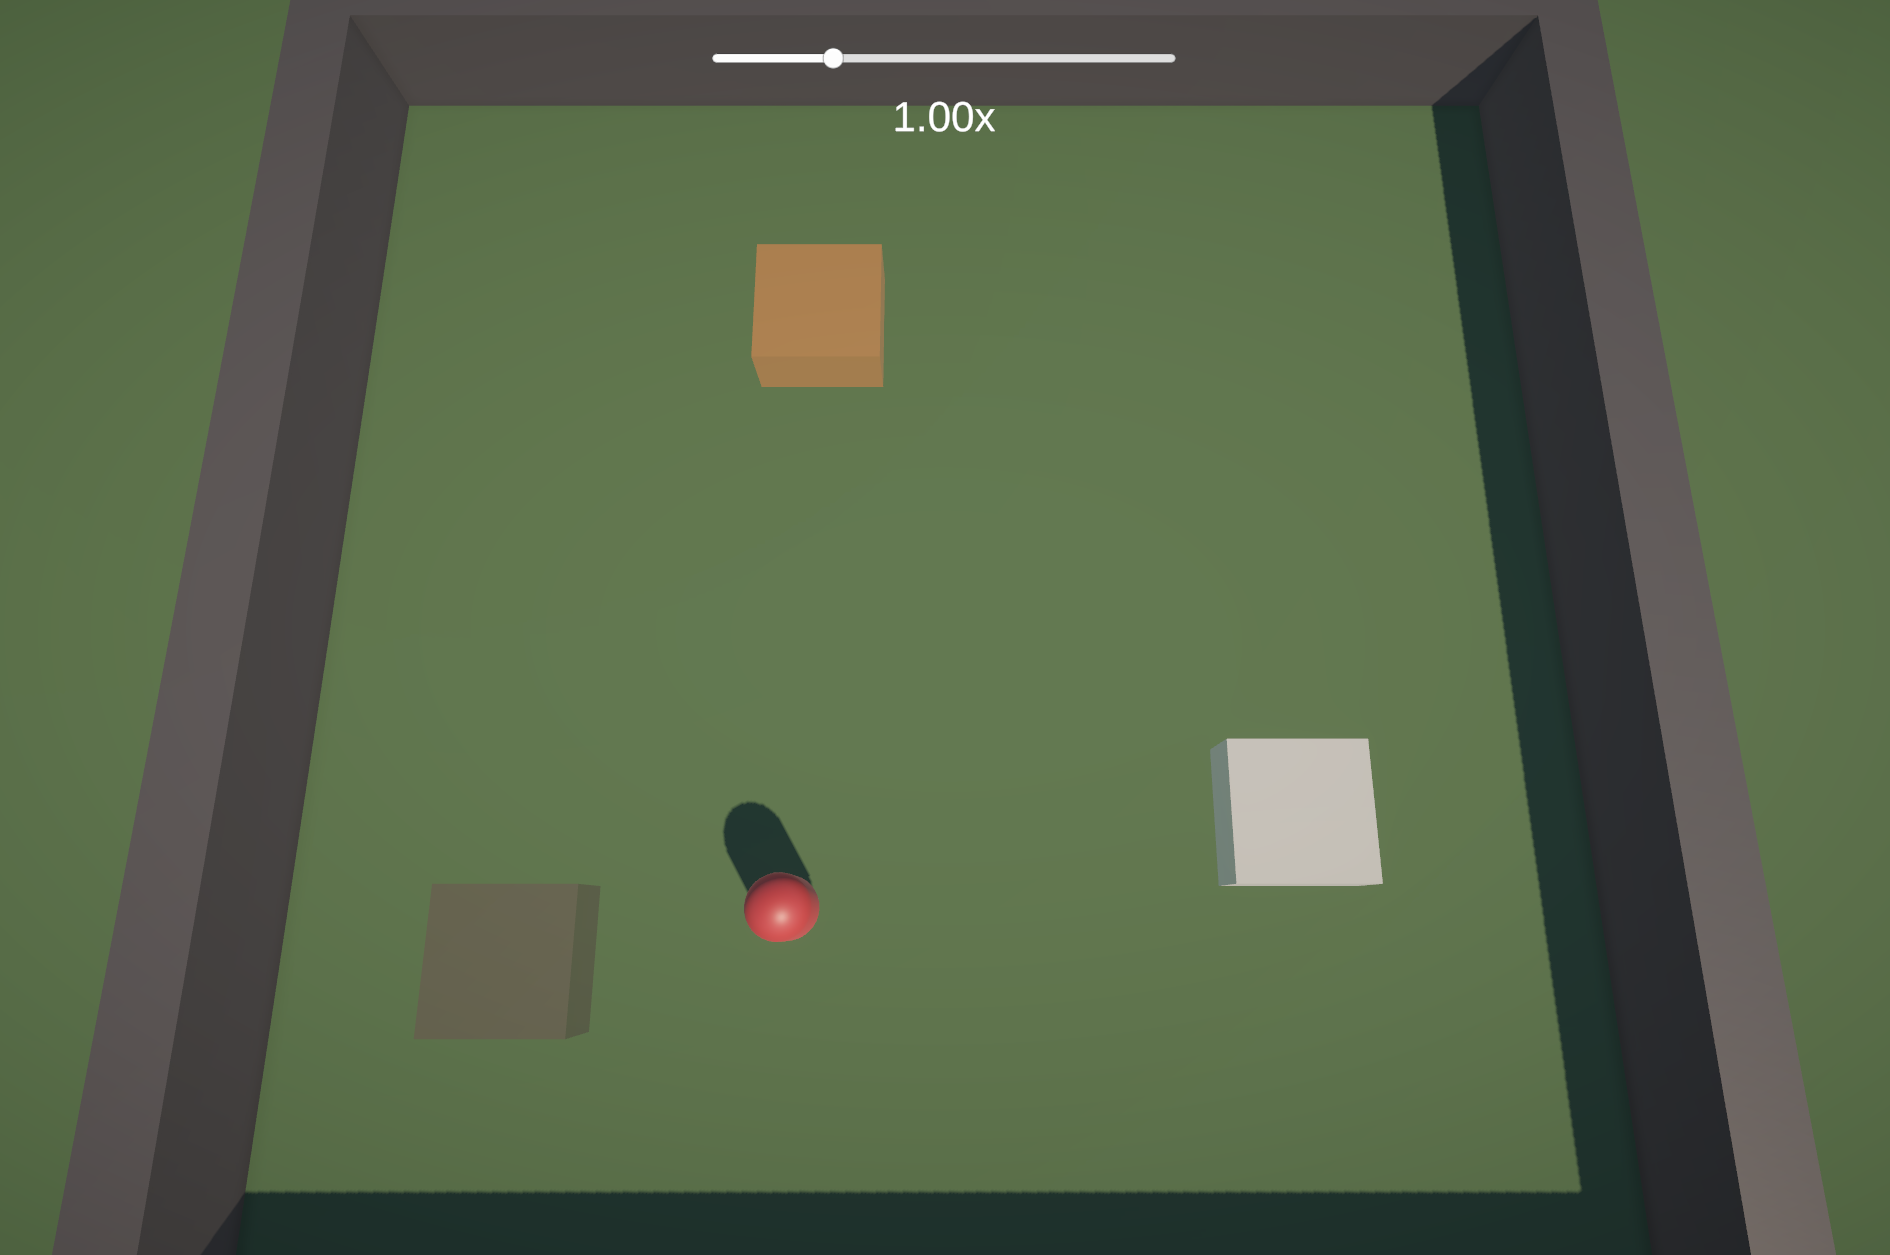
\includegraphics[scale=0.2]{images/utility_designer_daily_routine.png}
	\caption{Scene in Unity for the agent's daily routine}
	\label{fig:utility_designer_daily_routine}
\end{figure}

\newpage

The behaviour for this scene using Utility Designer is as follows:

\begin{figure}[H]
	\centering
		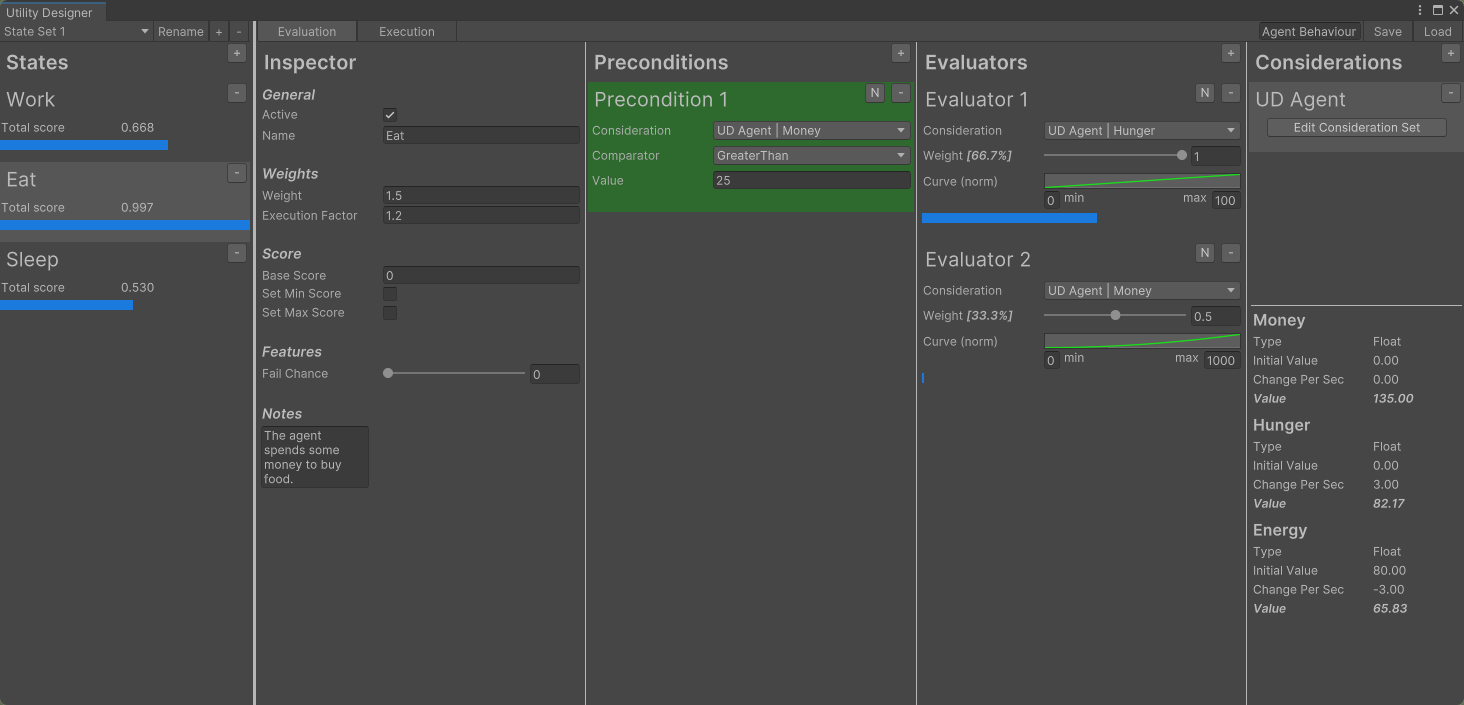
\includegraphics[scale=0.38]{images/utility_designer_daily_routine_evaluation.png}
	\caption{Evaluation tab for the agent in Utility Designer}
	\label{fig:utility_designer_daily_routine_evaluation}
\end{figure}

The figure \ref{fig:utility_designer_daily_routine_evaluation} shows the evaluation tab with the "Eat" state selected. This state is evaluated using hunger and money, with hunger having twice the weight of money. To eat, the agent must have at least enough money to buy one meal.

\begin{figure}[H]
	\centering
		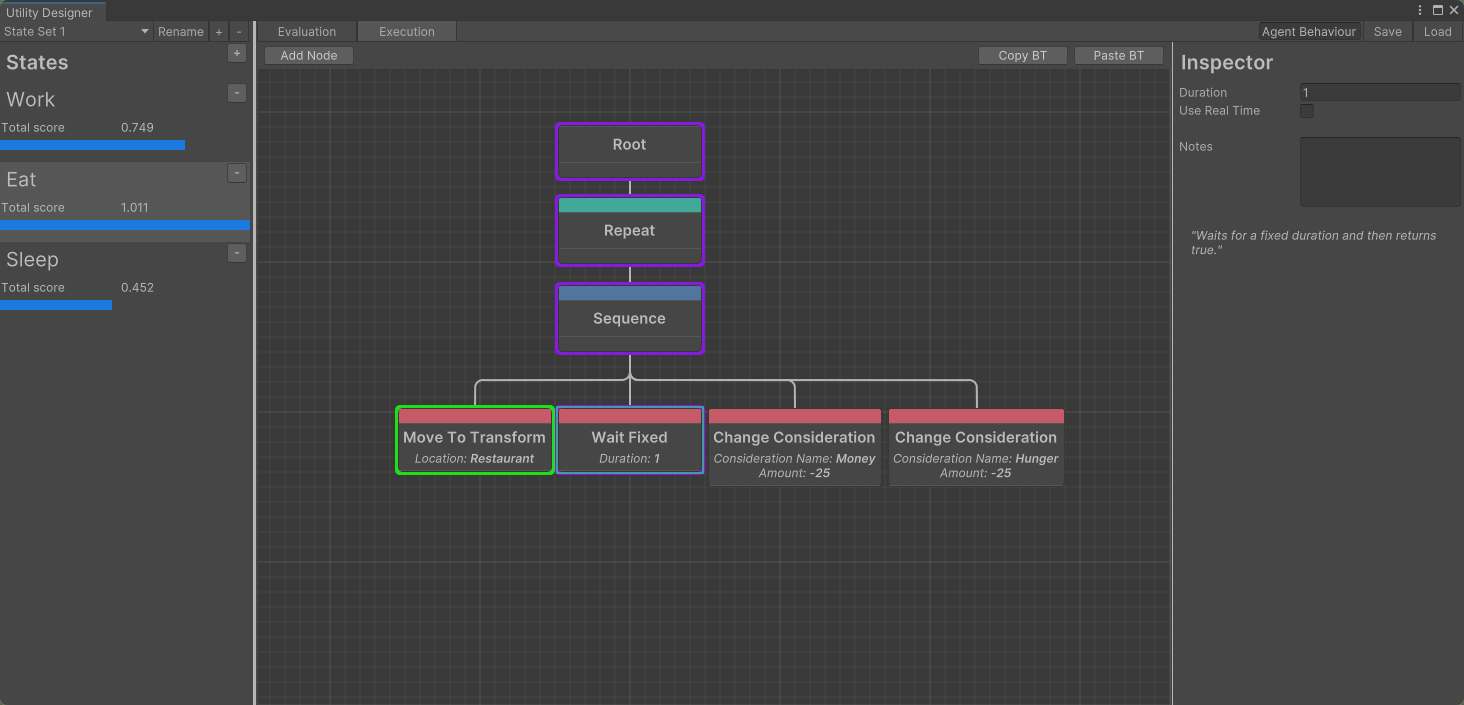
\includegraphics[scale=0.38]{images/utility_designer_daily_routine_execution.png}
	\caption{Execution tab for the agent in Utility Designer}
	\label{fig:utility_designer_daily_routine_execution}
\end{figure}

The Execution tab looks fairly straightforward. There is only one repeating sequence, which makes the agent go to the restaurant if he has not already done so, and pay 25 money to lose 25 hunger, repeated every second. The other states look pretty similar, just changed to suit the state.

\newpage

\subsection{Survival}
\label{sec:utilitydesigner_implementation_examplescenes_survival}

In the survival scene, the NPC called James has to survive as long as possible by efficiently choosing which task is best given the current circumstances. James will die either by being eaten by a bear or by starvation. James has the following states:

\begin{tabular}{lp{12cm}}
Fish: & Gets food slowly at a random rate and is always successful. \cr
Hunt: & Attempts to kill a deer to get a lot of food quickly, but the chance of success decreases the less energy and strength he has. Needs a deer nearby. \cr
Sleep: & Takes a nap to restore energy over time. \cr
Eat: & Roasts and eats meat from fishing and hunting to reduce hunger. \cr
Work out: & Builds up strength over time. Cannot be done if motivation is too low. Reduces motivation and energy. \cr
Fight: & Sometimes a bear will attack him. Will die if he does not have enough strength. \cr
Play: & Increases motivation over time. Cannot play if too hungry. \cr
\end{tabular}

Two different consideration sets were used to evaluate the states. One is specific to the needs and desires of James, and a global one is used to represent the environment. The consideration set for James is local, because it is specific to each instance of James, if there were more than one. It contains the considerations "Hunger", "Energy", "Food", "Motivation" and "Strength". The consideration set about the environment only has two considerations: "Deer nearby" and "Bears nearby".

The scene was created using the Low Poly Ultimate Pack Asset, which contains many low-poly pre-built assets to help create decent-looking scenes quickly.

\begin{figure}[H]
	\centering
		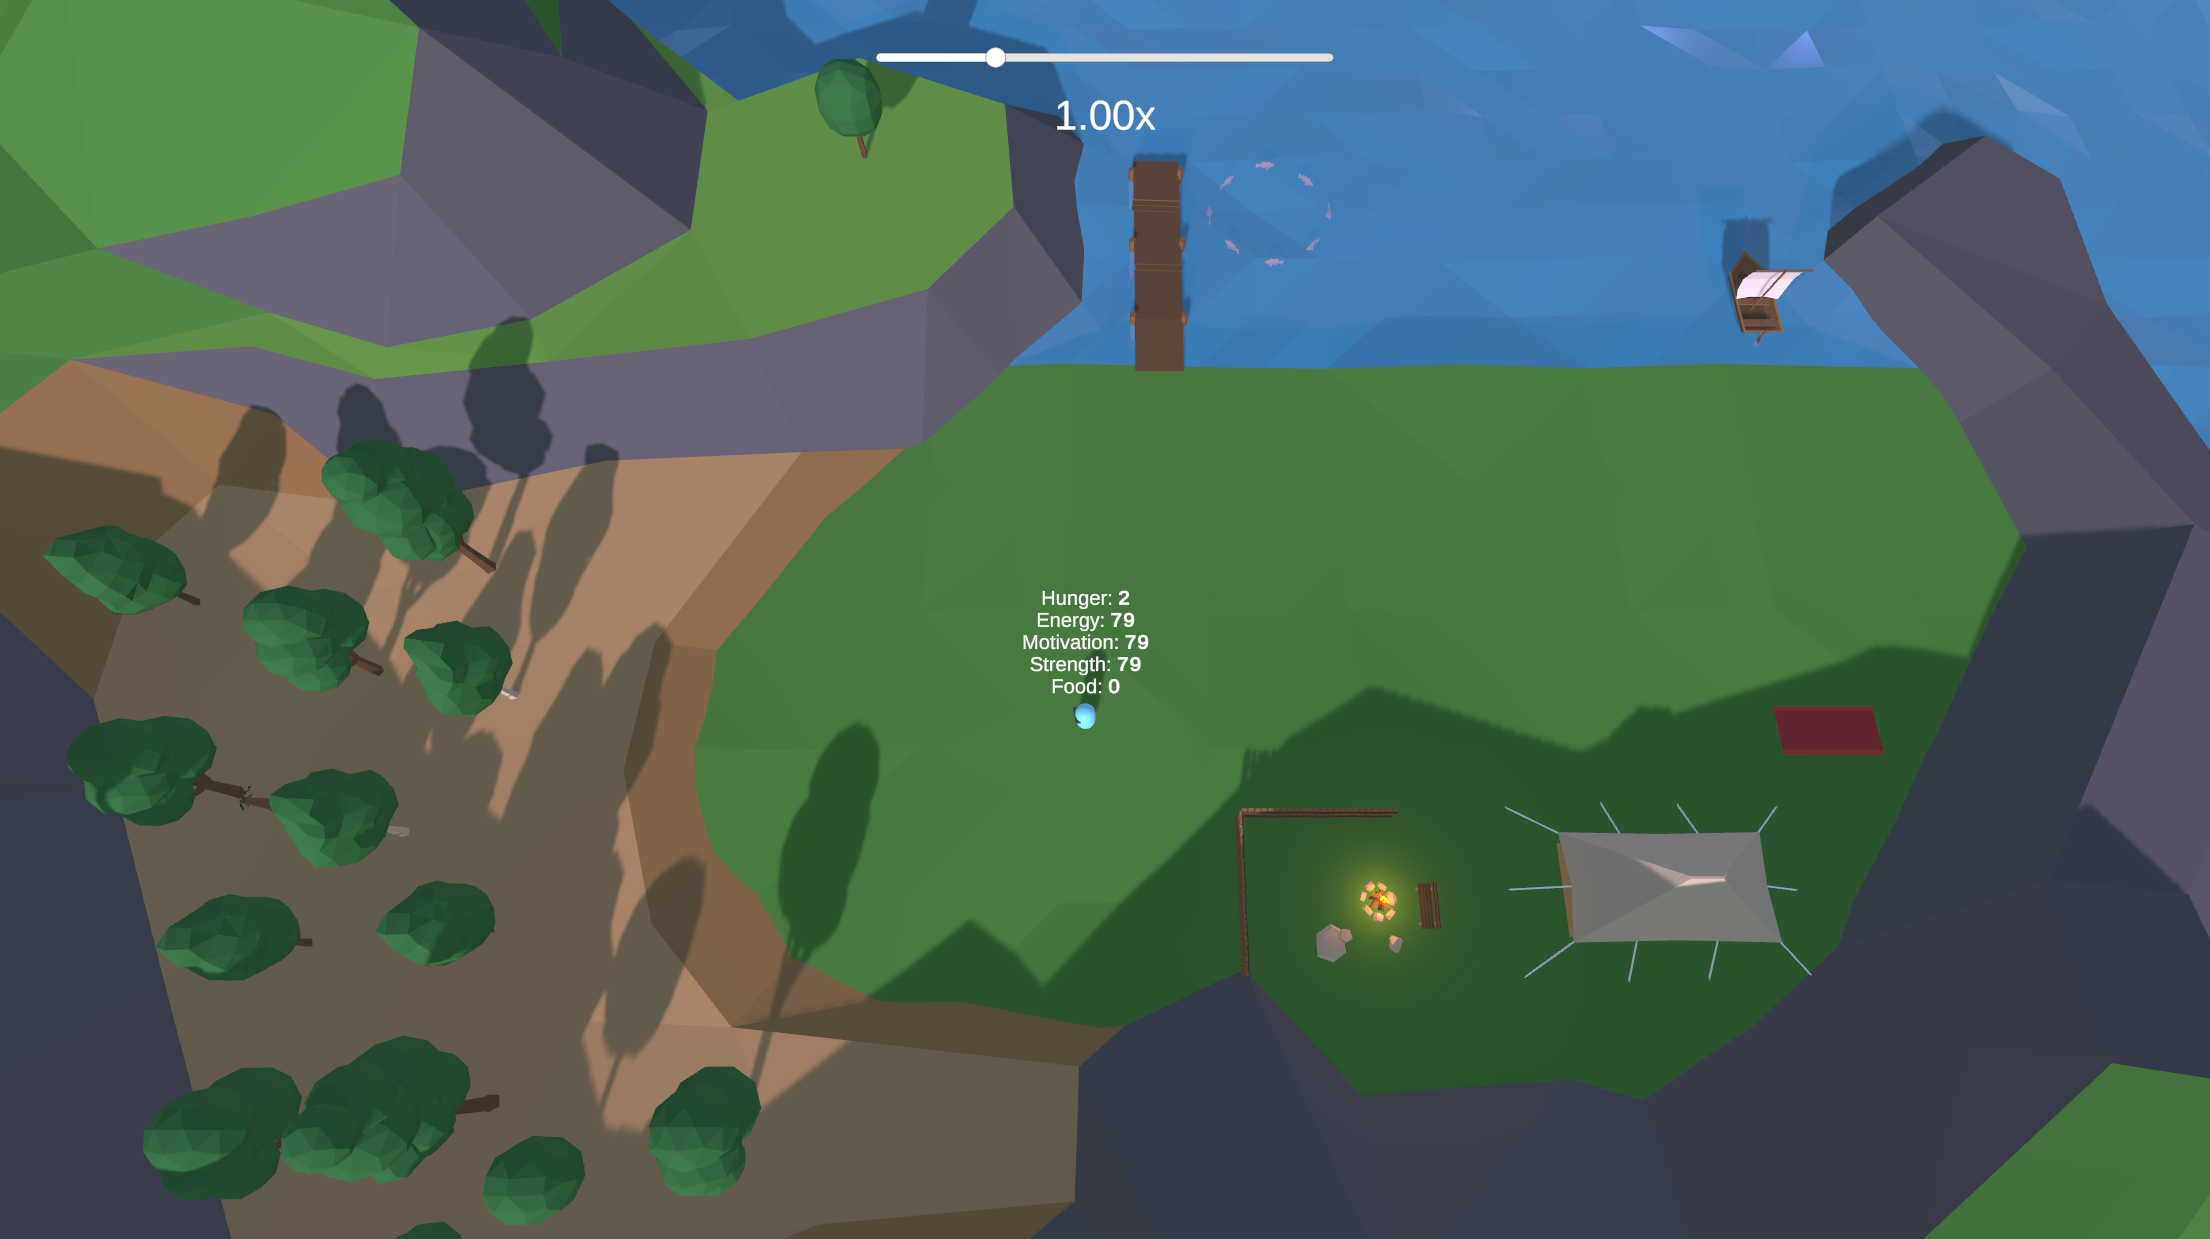
\includegraphics[scale=0.25]{images/utility_designer_survival.png}
	\caption{Survival scene in Unity}
	\label{fig:utility_designer_survival}
\end{figure}

\begin{figure}[H]
	\centering
		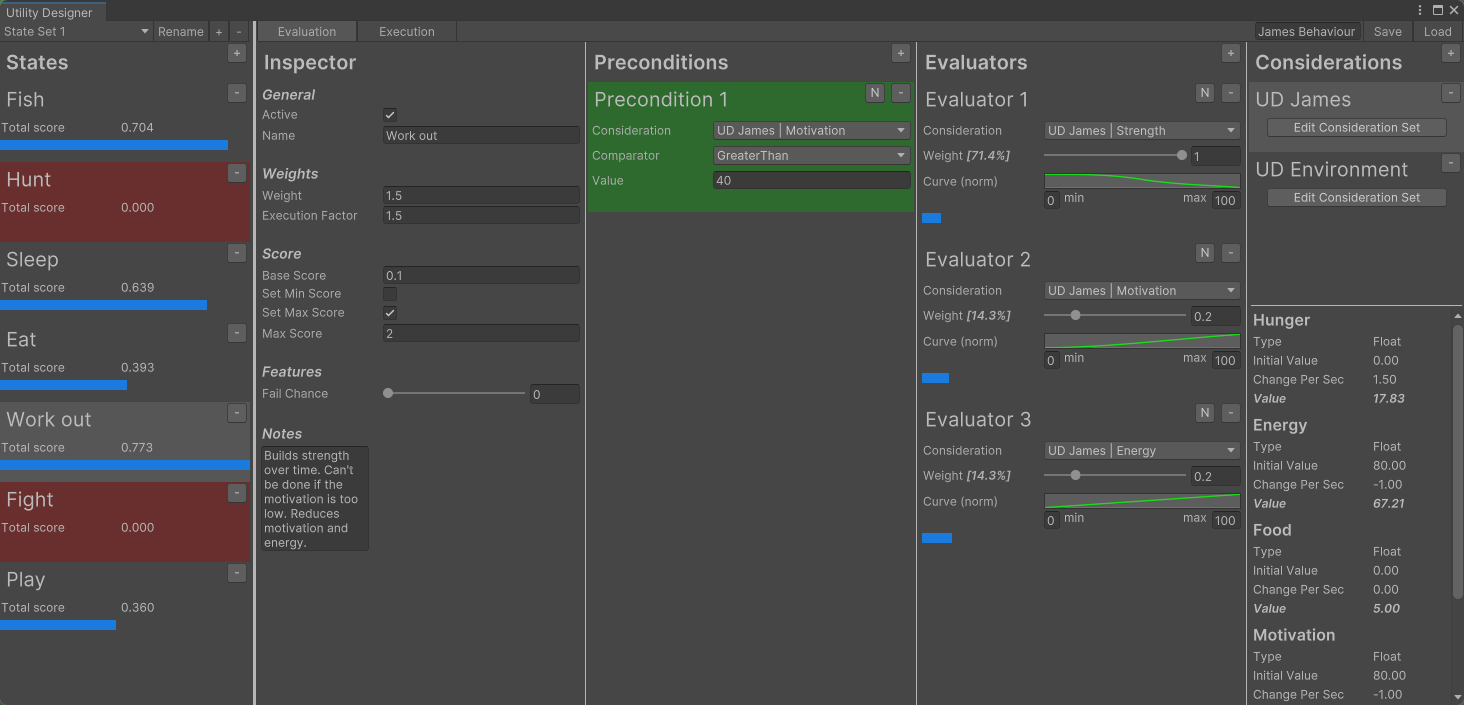
\includegraphics[scale=0.38]{images/utility_designer_survival_evaluation.png}
	\caption{Evaluation tab of Utility Designer}
	\label{fig:utility_designer_survival_evaluation}
\end{figure}

In the figure \ref{fig:utility_designer_daily_routine_evaluation}, the "Work out" state is currently selected and evaluated based on James' strength, motivation and energy. The most important factor for James is his own strength, as he would die from a bear attack if he was too weak. However, James does not like to train when he feels demotivated or tired, so evaluators 2 and 3 have a weight of 0.2. He also refuses to train when his motivation is very low, hence the precondition. The whole state is quite important, as he needs strength to survive a bear attack, which is represented by a weight of 1.5 and a base score of 0.1.

\begin{figure}[H]
	\centering
		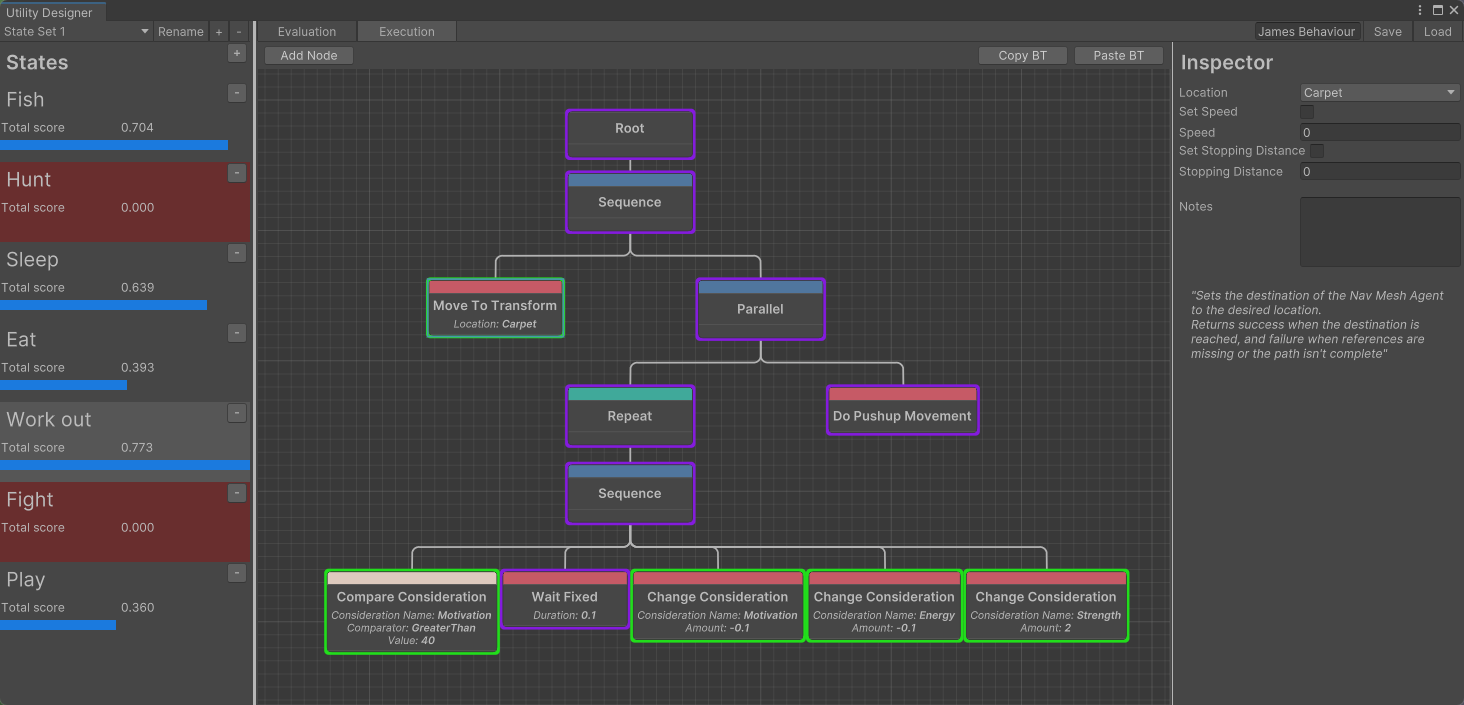
\includegraphics[scale=0.38]{images/utility_designer_survival_execution.png}
	\caption{Execution tab of Utility Designer}
	\label{fig:utility_designer_survival_execution}
\end{figure}

This shows the behaviour tree for the "Work out" state again. the first sequence is used to move to the carpet if it is not already there. Then the work out starts with a parallel node that allows the push up animation to be executed and the considerations to be changed in parallel. To the left of the sequence is a conditional node that checks whether James is motivated enough or not. This node is not really needed, as this condition is already checked in the evaluation tab, but it is here to show that such a check might also be possible in the behaviour tree. If this check is successful, the agent will gain 2 strength at a cost of 0.1 motivation and energy every 0.1s.

There were many variables that had to be set to make the NPC behave correctly, such as all the weights for the evaluators, adding preconditions, and configuring the inspector. But it was not as hard to configure as one might think, because everything can be done by intuition and simply thinking about the overall importance of each state and evaluator to get appropriate weights. Of course, some test runs were needed to fine-tune everything, which was also not too difficult due to the runtime debugging features.